\documentclass[a4paper]{article}
\usepackage[utf8]{inputenc}
\usepackage[T1]{fontenc}
\usepackage{inter}
\usepackage{parskip}
\usepackage{graphicx}
\usepackage{setspace}
\usepackage{lettrine}
\usepackage{fancyhdr}
\usepackage[portuguese]{babel}
\usepackage{xcolor}
\usepackage{minted}

\renewcommand{\baselinestretch}{1.5}

\fancyhf{}
\renewcommand{\headrulewidth}{0pt}
\rfoot{\thepage}
\definecolor{LightGray}{gray}{0.9}
\pagestyle{fancy}

\color{darkgray}
\usemintedstyle{pastie}

\begin{document}
    \renewcommand{\contentsname}{SUMÁRIO}
    \tableofcontents
    \newpage

    \subsection{Resumo}\label{subsec:resumo}
    Este relatório documenta a implementação e a avaliação de cinco algoritmos de ordenação implementados em C. Os algoritmos Bubble Sort, Selection Sort, Insertion Sort, Quick Sort e Heap Sort, tiveram suas eficiencias comparadas. Ao fim, foram criados gráficos que
    demonstram as diferenças dos algoritmos em termos de tempo de execução, número de comparações e número de trocas para vetores aleatórios.
    O trabalho foi em dupla, mas os relatórios foram feitos individualmente.
    Realizei este trabalho com Vínicius Roberto Valentini, de matrícula \textbf{\textit{2311100041} }.


    \section{Metodologia}\label{sec:metodologia}
    \subsection{Alocação e seleção dos números e algoritmos}\label{subsec:alocacao-e-selecao-dos-numeros}
    Para realizar o trabalho, foi preciso primeiro executar cada um dos algoritmos dentro de um for loop para cada tamanho especificado pela demanda do trabalho.
    Além disso, para cada valor, foram gerados valores aleatórios para que o experimento fosse de fato relevante e pudesse dizer a média nos piores casos, nos médios e nos melhores.
    Isso é demonstrado pela linha de código abaixo, onde inicia-se o loop e os valores do vetor são alocados e gerados.
    \begin{minted}[bgcolor=LightGray, fontsize=\footnotesize]{C}
     for (int i = 0; i < num_tamanhos; i++) {
        int tamanho_atual = tamanhos[i];
        printf("\nIniciando testes para vetores de tamanho %d...\n", tamanho_atual);

        // Todo o trabalho para um tamanho específico vai acontecer aqui dentro...

        int *vetor_original = (int *)malloc(tamanho_atual * sizeof(int));
        if (vetor_original == NULL) {
            printf("Falha ao alocar memoria. Abortando.\n");
            return 1;
        }
        for (int j = 0; j < tamanho_atual; j++) {
            // Função demorada se o vetor for grande demais
            vetor_original[j] = rand() % 10000;
        }
    \end{minted}

    Após a criação do vetor original com valores aleatórios para um determinado tamanho, o próximo passo foi executar cada um dos algoritmos de ordenação. Uma nova cópia do \texttt{vetor\_original} é alocada dinamicamente para cada algoritmo. A função \texttt{copia()} é usada para preencher esta cópia.
    Em seguida, cada algoritmo é chamado (como \texttt{bubbleSort}, \texttt{insertionSort}, etc.) um por um para ordenar a cópia.
    Ao final do loop, o \texttt{vetor\_original} também é liberado.

    \begin{minted}[bgcolor=LightGray, fontsize=\footnotesize]{C}
        //  Teste para o Bubble Sort
        int *copia_para_bubble = (int *)malloc(tamanho_atual * sizeof(int));
        copia(vetor_original, copia_para_bubble, tamanho_atual);
        bubbleSort(copia_para_bubble, tamanho_atual);
        free(copia_para_bubble);

        //  Teste para o Insertion Sort

        // Heapsort

        free(vetor_original);
    }
    \end{minted}

    \subsection{Salvamento dos dados}\label{subsec:salvamento-dos-dados}

    Para capturar e salvar os dados de performance de cada execução, foi implementado um sistema de escrita em arquivos binários. O núcleo desse sistema é a estrutura \texttt{Sort}, definida no arquivo \texttt{sorting.h} (ou \texttt{sorting.c}).

    Esta estrutura foi definida com o atributo \texttt{\_\_attribute\_\_((packed))}. Isso foi necessário para que a estrutura pudesse ser lida pelo Python corretamente, pois o Python esperava que a estrutura tivesse uma quantidade bem específica de bytes.


    \begin{minted}[bgcolor=LightGray, fontsize=\footnotesize]{C}
    // Foi necessário aplicar o packed pra facilitar a leitura pelo python
    // Python espera 26 bytes, mas sem o packed aqui fica 32 bytes
    typedef struct __attribute__((packed)) sort {
        char tipo[10];
        long long trocas;
        long long comparacoes;
        double tempo;
    } Sort;
    \end{minted}

    Uma função, \texttt{createSortItem}, é usada para criar um dado. Essa estrutura é usada para armazenar e passar
    todos os dados, como as trocas, as comparações e etc dentro de um arquivo binário. Ela será usada mais a frente.
    \begin{minted}[bgcolor=LightGray, fontsize=\footnotesize]{C}
    // Cria uma estrutura de sort com os detalhes
    Sort createSortItem(char* tipo, long long swaps, long long comparacoes, double tempo) {
    Sort sort;
    sort.trocas = swaps;
    sort.comparacoes = comparacoes;
    sort.tempo = tempo;
    memset(sort.tipo, 0, sizeof(sort.tipo));
    strncpy(sort.tipo, tipo, sizeof(sort.tipo)-1);
    return sort;
    }
    \end{minted}
    A escrita dos dados em disco é gerenciada pela função \texttt{writeSortingData}. Ela abre um arquivo binário para cada algoritmo (ex: \texttt{./executions/bubble.bin}) no modo \texttt{"ab"} (append binary). Este modo é crucial, pois ele adiciona novos dados ao \textit{final} do arquivo, preservando os registros das execuções anteriores (para tamanhos de vetores diferentes).
    Vale mencionar que em cada execução esses arquivos são apagados para que não misture-se dados antigos com dados novos.
    A função \texttt{fwrite} é usada para escrever os bytes puros da \texttt{struct Sort} diretamente no arquivo.


    \begin{minted}[bgcolor=LightGray, fontsize=\footnotesize]{C}
    // Adiciona as informações da execução n
    void writeSortingData(char* filename, Sort sort) {
        FILE *f = fopen(filename, "ab");
        if (f == NULL) {
            printf("Falhou ao abrir o arquivo '%s'.\n", filename);
            return;
        }
        printf("\nSalvando %s - Swaps: %lld - Comparações: %lld",
               sort.tipo, sort.trocas, sort.comparacoes );
        fseek(f, 0, SEEK_END);
        fwrite(&sort, sizeof(Sort), 1, f);
        fclose(f);
    }
    \end{minted}

    Dentro de cada função de ordenação (ex: \texttt{bubbleSort}), o algoritmo é executado 3 vezes. As métricas (trocas, comparações e tempo) são acumuladas e, ao final, uma \textit{média} é calculada. É essa média que é então passada para \texttt{createSortItem} e \texttt{writeSortingData} para ser salva.

    \begin{minted}[bgcolor=LightGray, fontsize=\footnotesize]{C}
        void bubbleSort(int *A, int size) {
            long long total_swaps = 0;
            long long total_comparisons = 0;
            double total_time = 0.0;
        
            // Executa 3 vezes para obter o tempo médio
            for (int exec = 0; exec < 3; exec++) {
                // ... (lógica do bubble sort) ...
                // ... (contagem de swaps, comparisons, tempo) ...
            }
        
            // Calcula as médias
            double tempo = total_time / 3.0;
            long long avg_swaps = total_swaps / 3;
            long long avg_comparisons = total_comparisons / 3;
        
            // Salva a média no arquivo binário
            writeSortingData("./executions/bubble.bin", 
              createSortItem("bubble", avg_swaps, avg_comparisons, tempo));
        }
    \end{minted}

    \subsection{Criação dos gráficos}\label{subsec:criacao-dos-graficos}
    Este processo resulta em cinco arquivos binários (um para cada algoritmo), onde cada arquivo contém uma sequência de \texttt{Sort} structs, representando a performance média para cada tamanho de vetor testado.
    Todo esse processo acontece após executar main.py.
    O arquivo em Python dá um \textbf{make} na Makefile dentro do arquivo de pastas, executa o arquivo em C, e então, ao estar completo, interpreta e constroi os gráficos usando a biblioteca do Python, Matplotlib.

    % Figures: tempo, comparacoes, trocas
    \begin{figure}[htbp]
      \centering
      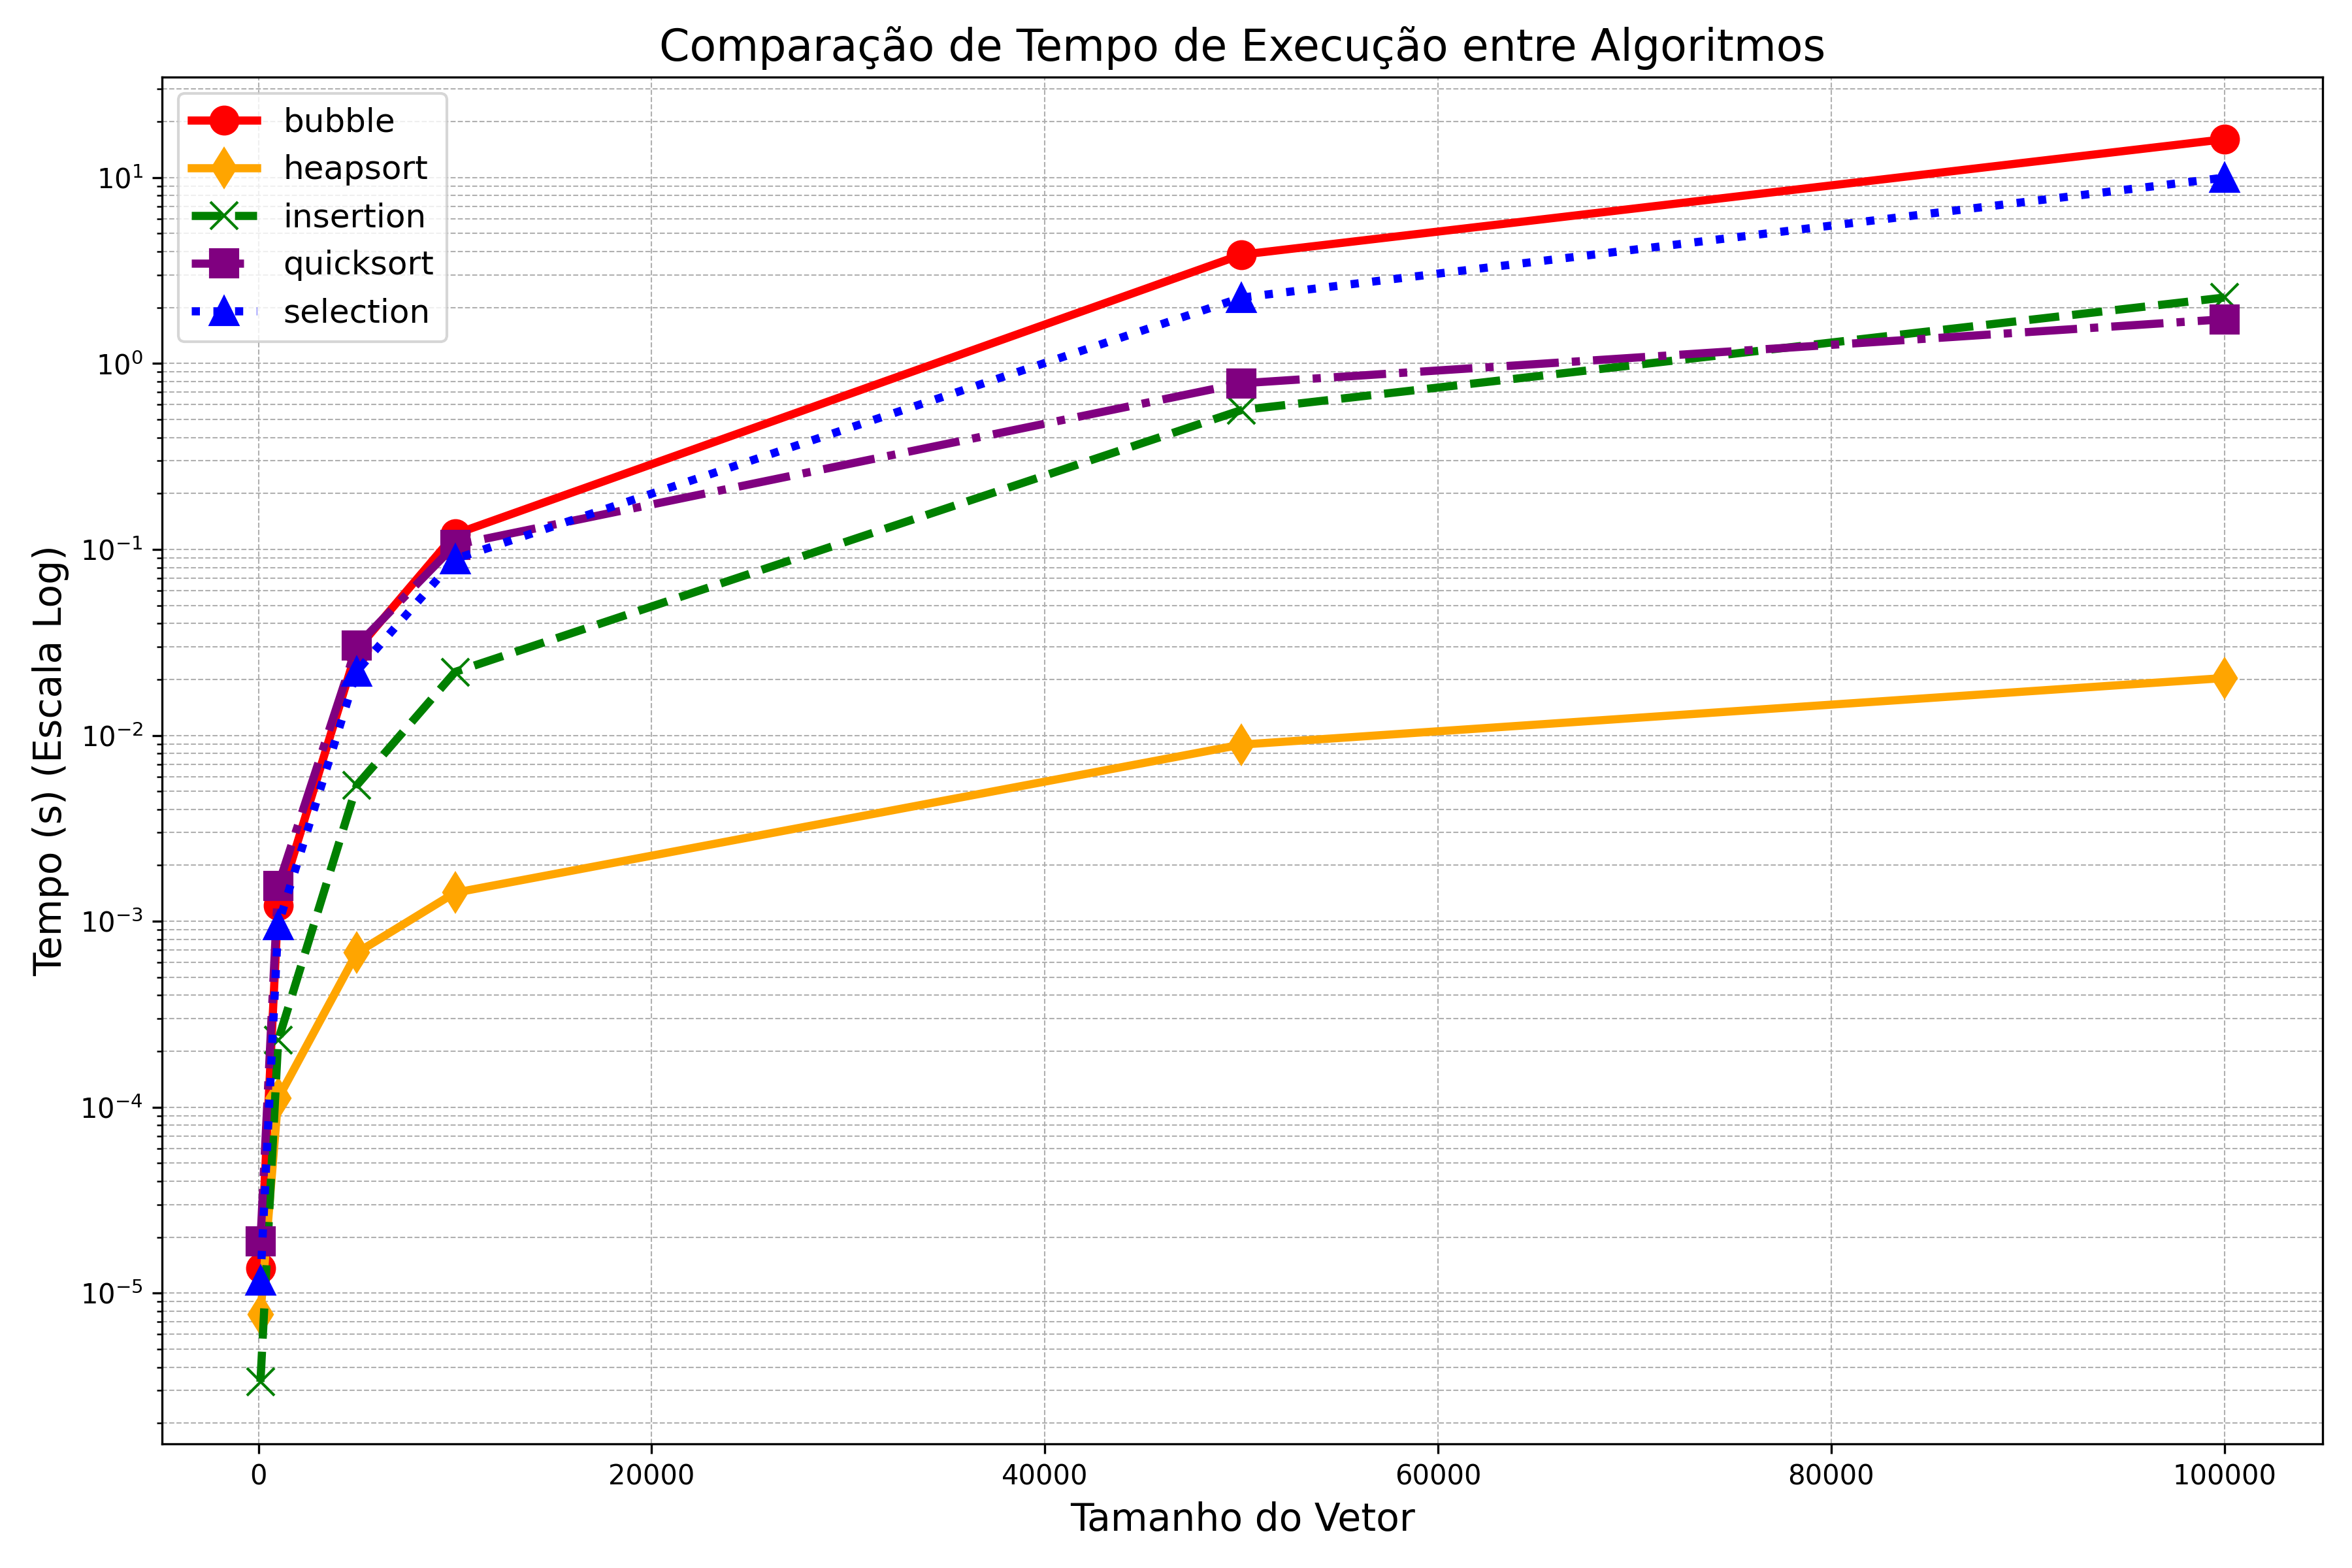
\includegraphics[width=0.9\textwidth]{../../graficos/tempo_comparacao}
      \caption{Comparação do tempo de execução entre os algoritmos (média sobre as execuções).}
      \label{fig:tempo_comparacao}
    \end{figure}

    \begin{figure}[htbp]
      \centering
      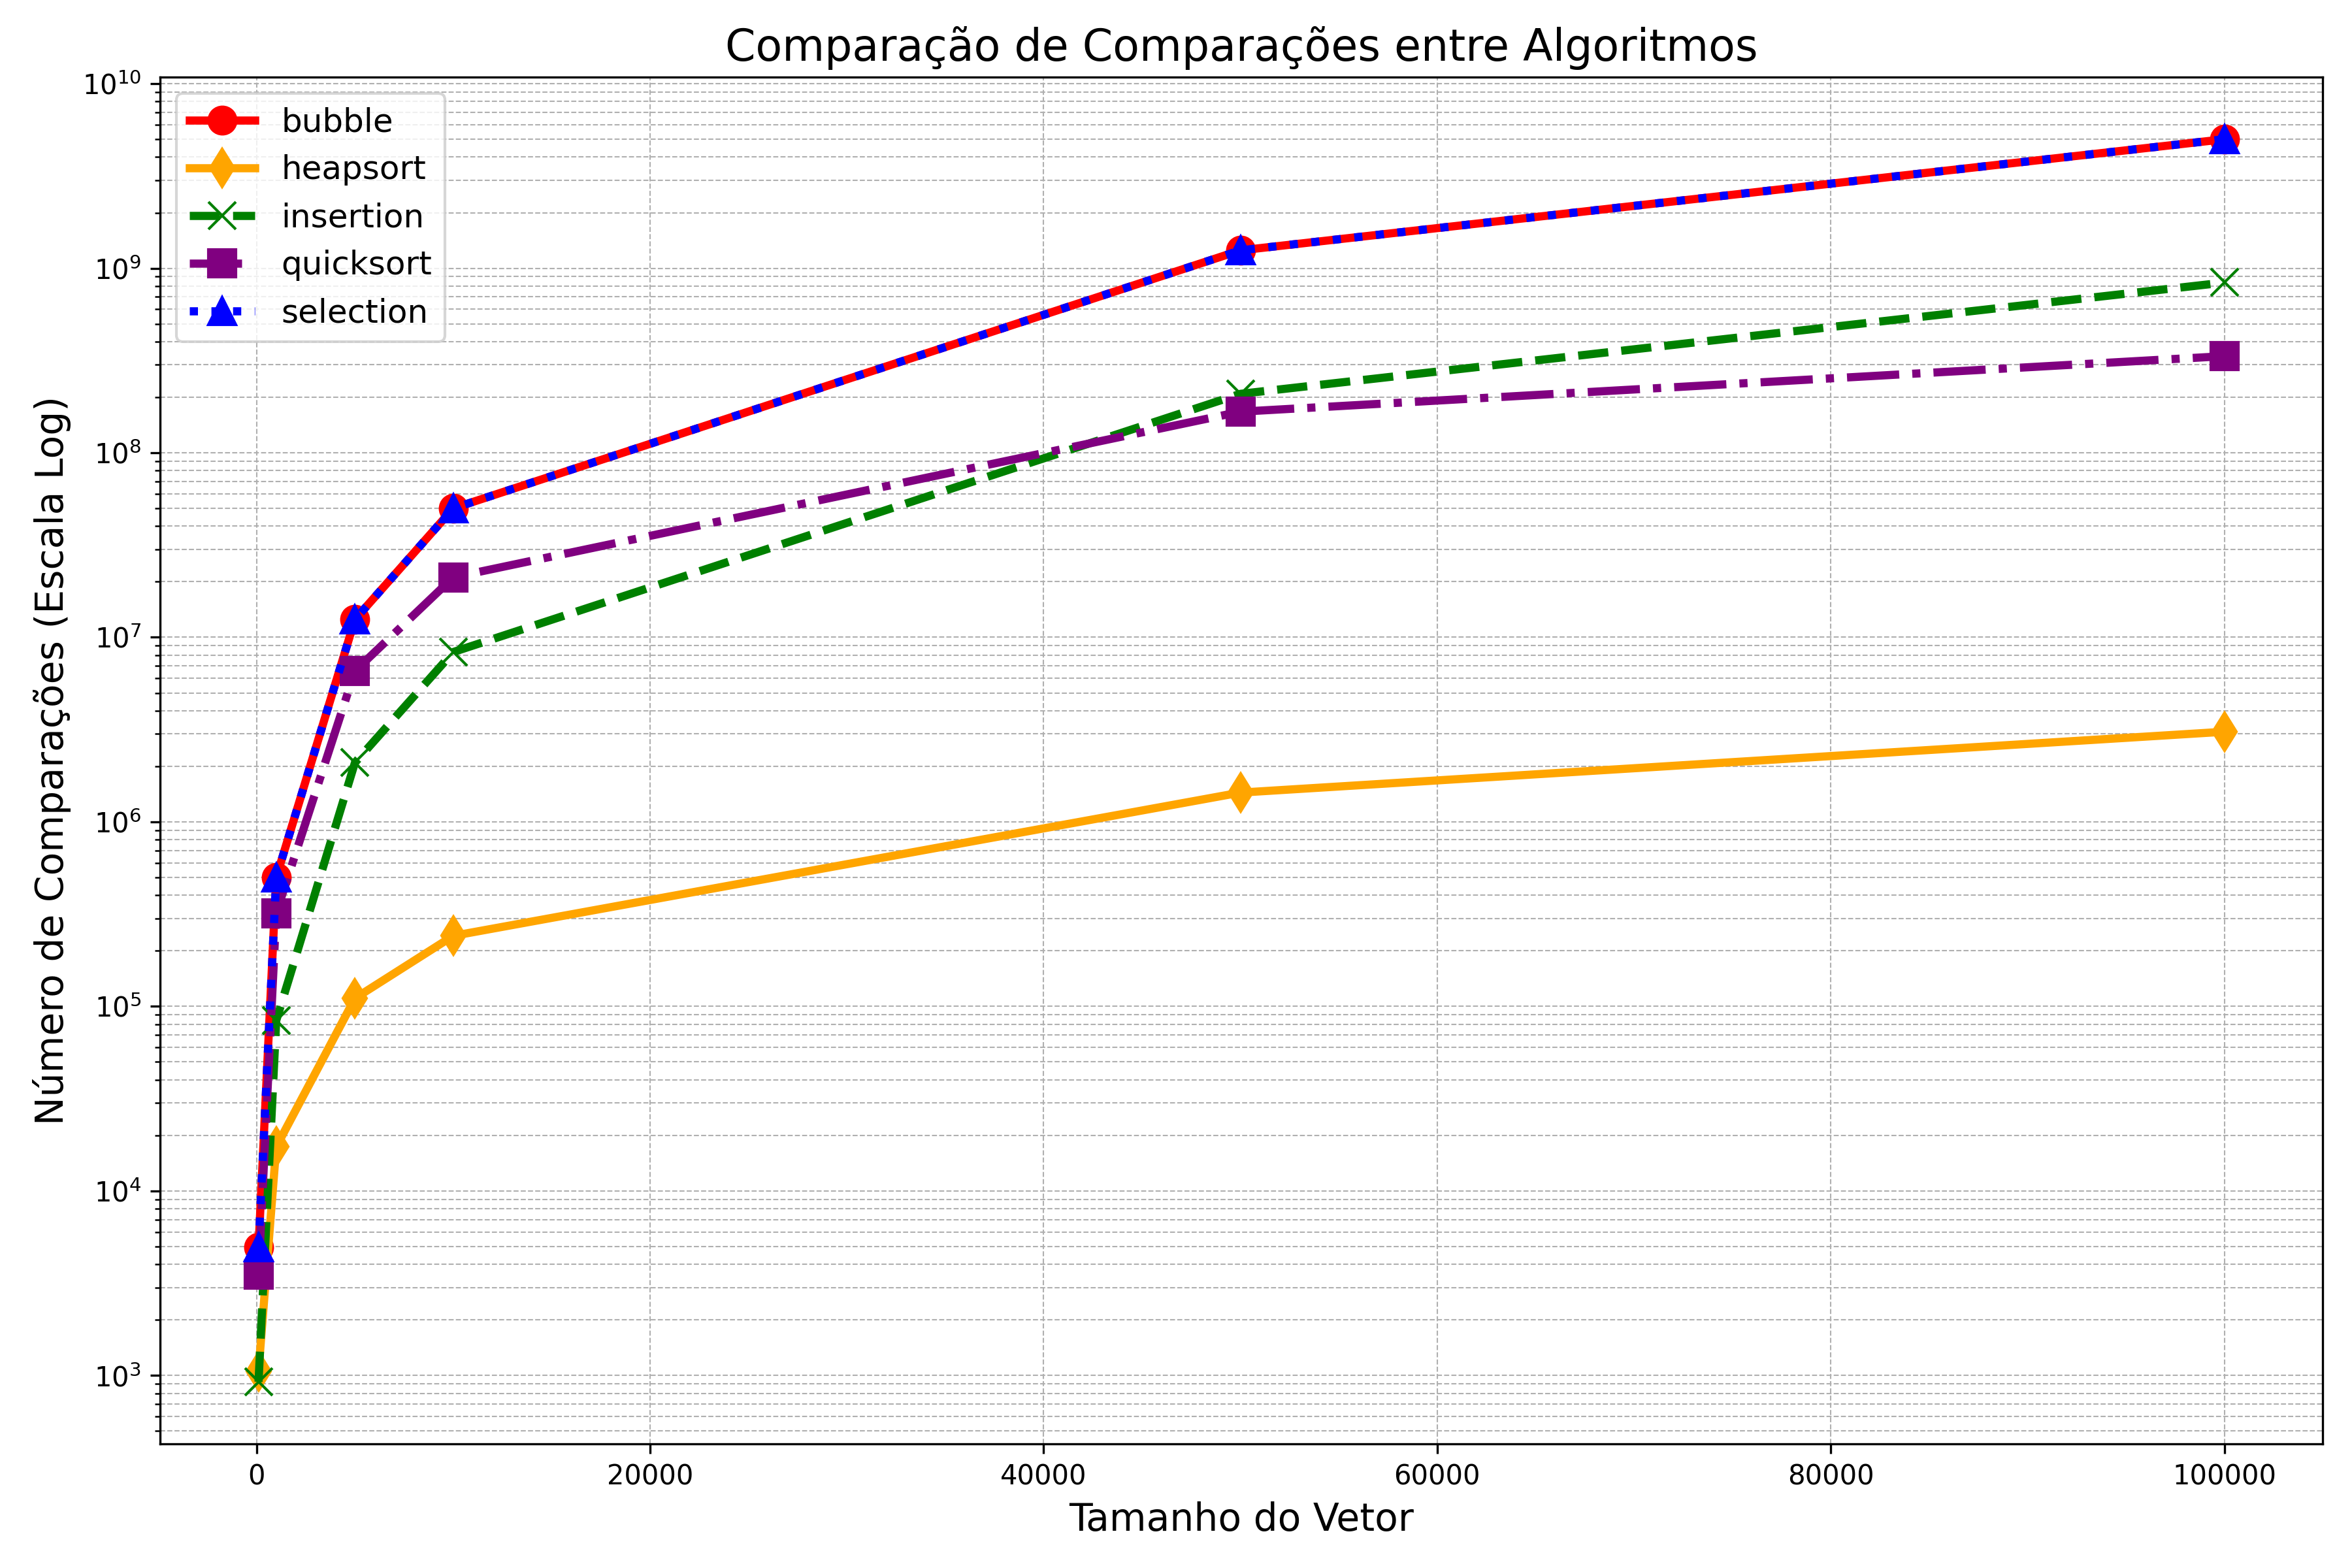
\includegraphics[width=0.9\textwidth]{../../graficos/comparacoes_comparacao}
      \caption{Número médio de comparações por algoritmo e por tamanho de entrada.}
      \label{fig:comparacoes_comparacao}
    \end{figure}

    \begin{figure}[htbp]
      \centering
      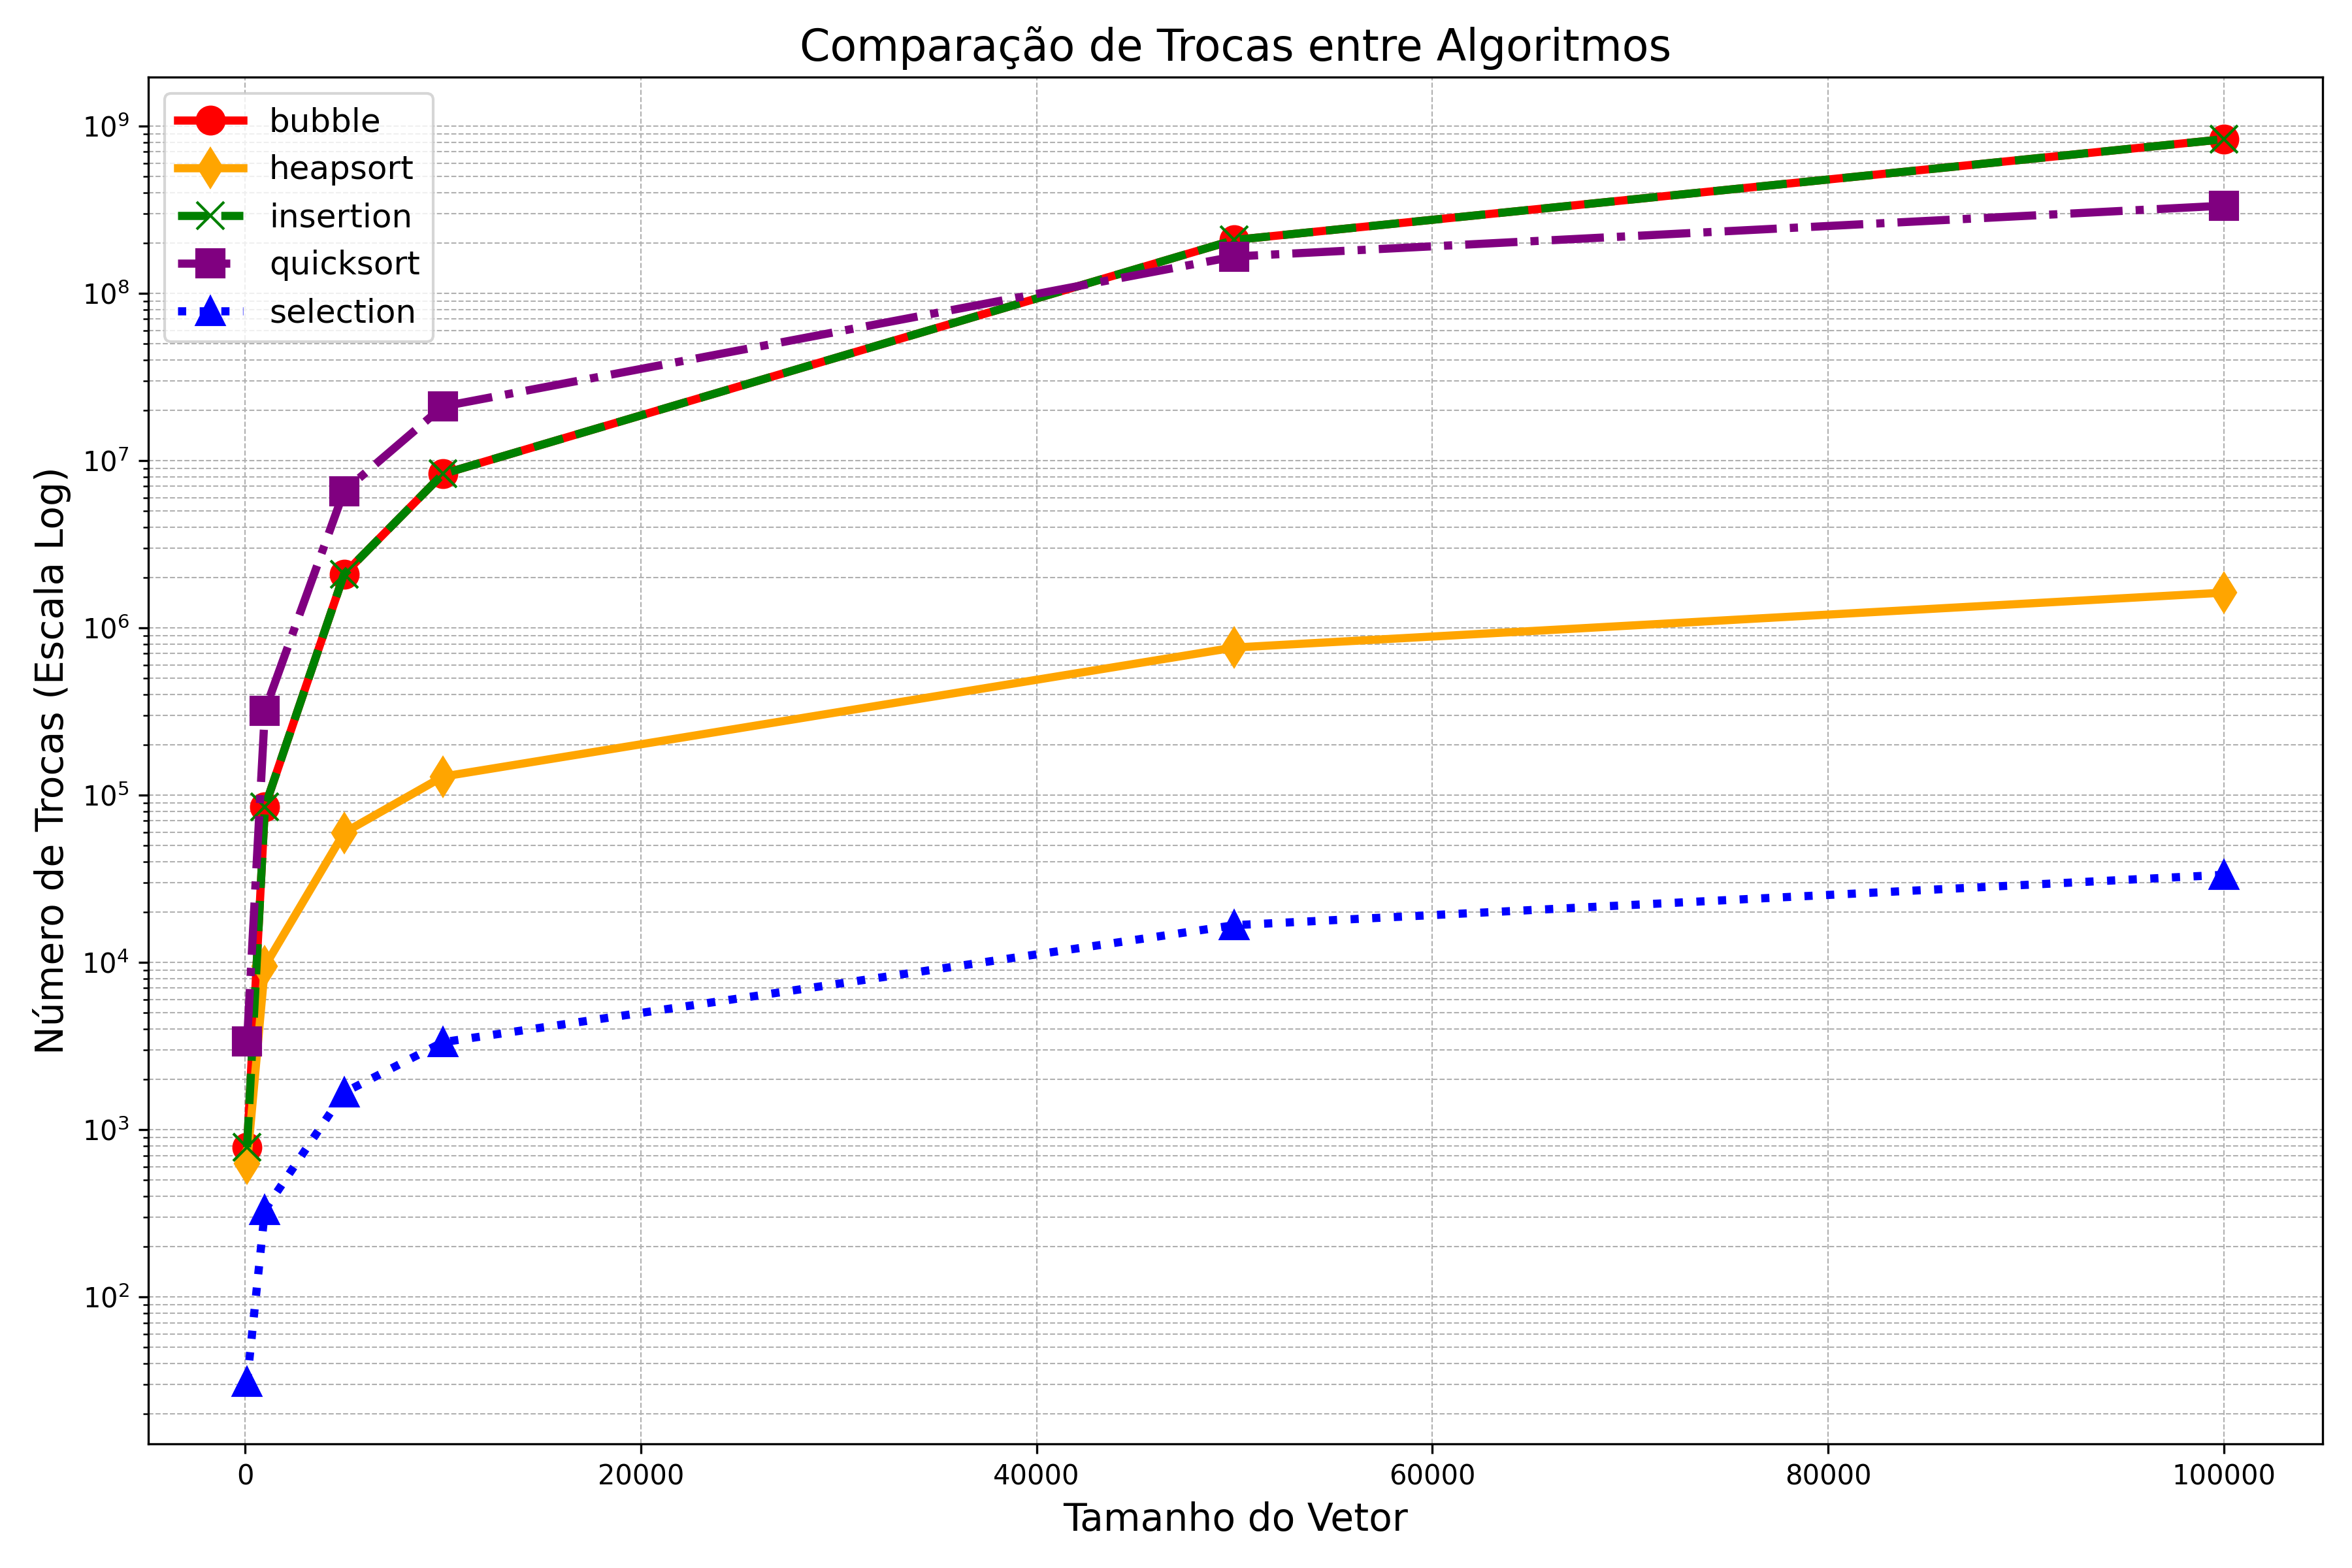
\includegraphics[width=0.9\textwidth]{../../graficos/trocas_comparacao}
      \caption{Número médio de trocas por algoritmo e por tamanho de entrada.}
      \label{fig:trocas_comparacao}
    \end{figure}

    \section{Funcionamento dos algoritmos}\label{sec:funcionamento-dos-algoritmos}

    A diferença de performance entre os algoritmos foi notável, especialmente em vetores grandes (N=100.000).

    Em termos de \textbf{Tempo de Execução}, o \textbf{Heap Sort} foi o mais eficiente, terminando em aproximadamente 0.02 segundos, o que era esperado de um algoritmo $O(n \log n)$. O \textbf{Quick Sort} (1.73s) e o \textbf{Insertion Sort} (2.29s) foram significativamente mais lentos, mas ainda muito mais rápidos que os algoritmos quadráticos ($O(n^2)$). O \textbf{Selection Sort} (9.92s) e o \textbf{Bubble Sort} (17.37s) demonstraram ser os mais lentos para este volume de dados.

    Para o \textbf{Número de Comparações}, o \textbf{Heap Sort} manteve sua liderança, necessitando de apenas 3 milhões de comparações. Em contraste, o \textbf{Quick Sort} ($\approx 334$ milhões) e o \textbf{Insertion Sort} ($\approx 833$ milhões) realizaram um número muito maior de verificações. O pior desempenho foi o do \textbf{Bubble Sort} e \textbf{Selection Sort}, ambos exigindo cerca de 5 bilhões de comparações, um comportamento típico de algoritmos quadráticos.

    No \textbf{Número de Trocas}, o \textbf{Selection Sort} foi o vencedor, realizando apenas 33 mil trocas.
    Isso é uma característica fundamental do seu design, que minimiza as operações de escrita na memória. O \textbf{Heap Sort} ficou em segundo lugar com 1.6 milhão de trocas. Os demais algoritmos, como Quick Sort e Bubble Sort, tiveram um custo muito maior em movimentação de dados, na casa das centenas de milhões.

    Concluindo a análise, o \textbf{Heap Sort} mostrou o melhor desempenho geral, sendo o mais rápido e o mais econômico em comparações. O \textbf{Quick Sort} foi competitivo em tempo de execução, mas teve um custo elevado de trocas e comparações. O \textbf{Selection Sort} brilha ao minimizar as trocas, mas seu alto número de comparações o torna lento. Por fim, \textbf{Bubble Sort} e \textbf{Insertion Sort} (quando aplicado a dados aleatórios) mostraram-se ineficientes para lidar com grandes volumes de dados.
    Vale mencionar que apesar do trabalho não pedir os três dados, eu achei que seria interessante fazer o gráfico dos números de comparações junto com o número de trocas.

    \subsection{Bubble Sort}\label{subsec:bubble-sort}
    O Bubble Sort percorre o vetor várias vezes.
    Em cada passagem, ele compara elementos vizinhos e os troca se estiverem fora de ordem.
    \begin{enumerate}
        \item Inicia um loop que percorre todo o vetor.
        \item Dentro dele, outro loop percorre o vetor novamente, comparando o elemento atual com o próximo.
        \item Se o elemento atual for maior que o próximo, eles trocam de lugar.
        \item Isso ocorre até o algoritmo estar ordenado, e por isso demora muito, como demonstram os gráficos e os resultados do trabalho.
    \end{enumerate}

    \subsection{Selection Sort}\label{subsec:selection-sort}
    O Selection Sort divide o vetor em uma parte ordenada (à esquerda) e uma desordenada (à direita).
    \begin{enumerate}
        \item O algoritmo percorre a parte desordenada para encontrar o menor elemento.
        \item Após encontrar o menor elemento, ele o troca com o primeiro elemento da parte desordenada.
        \item Isso move o menor elemento para a parte ordenada.
        \item O processo é repetido, começando da segunda posição, depois da terceira, até que todo o vetor esteja ordenado.
        \item Sua principal característica é minimizar o número de trocas.
    \end{enumerate}

    \subsection{Insertion Sort}\label{subsec:insertion-sort}
    O Insertion Sort também mantém uma parte ordenada à esquerda.
    Ele pega um elemento da parte desordenada e o insere no lugar certo da parte ordenada.
    \begin{enumerate}
        \item Começa pelo segundo elemento do vetor (assumindo que o primeiro já é uma "lista ordenada" de um item).
        \item Salva o elemento atual como chave.
        \item Olha para trás, para os elementos na parte ordenada.
        \item Se o elemento anterior for menor que a chave, ele manda para o lado. E assim continua.
        \item O algoritmo continua olhando para trás e empurrando elementos até encontrar a posição correta.
        Isso pode ser um elemento maior ou o final do vetor.
        \item Repete o processo para todos os outros elementos da parte desordenada.
    \end{enumerate}

    \subsection{Quick Sort}\label{subsec:quick-sort}
    \begin{enumerate}
        \item Primeiro, ele escolhe um elemento do vetor para ser o pivô.
        \item Todos os elementos menores que o pivô são movidos para sua esquerda, e os maiores para sua direita.
        \item O pivô é colocado em sua posição final correta.
        \item Agora, o pivô está ordenado.
        \item O algoritmo então repete esse mesmo processo.
        \item Faz o mesmo para a sub-lista à direita do pivô e à esquerda.
        \item Isso continua dividindo o vetor em partes menores até que tudo esteja ordenado.
    \end{enumerate}

    \subsection{Heap Sort}\label{subsec:heap-sort}
    \begin{enumerate}
        \item \textbf{Fase 1: Construir o Heap}
        \item O algoritmo primeiro transforma o vetor inteiro em um Max Heap.
        A função \texttt{heapify} é usada para garantir que cada pai seja maior que seus filhos.
        \item Ao final desta fase, o maior elemento de todo o vetor está na primeira posição.
        \item \textbf{Fase 2: Ordenar}
        \item O algoritmo troca o primeiro elemento com o último elemento do vetor.
        \item O último elemento está agora em sua posição final e ordenada.
        \item A troca provavelmente quebrou a regra do Max Heap na raiz.
        O algoritmo chama \texttt{heapify} novamente na raiz (posição 0) para empurrar o elemento para baixo e consertar a estrutura.
        \item Isso continua até o vetor estar ordenado.
    \end{enumerate}

\end{document}